%\documentclass{article}
%
%\usepackage{fancyhdr}
%\usepackage{extramarks}
%\usepackage{amsmath}
%\usepackage{amsthm}
%\usepackage{amsfonts}
%\usepackage{tikz}
%\usepackage{enumerate}
%\usepackage{graphicx}
%\graphicspath{ {images/} }
%\usepackage[plain]{algorithm}
%\usepackage{algpseudocode}
%\usepackage[document]{ragged2e}
%\usepackage{textcomp}
%\usepackage{color}   %May be necessary if you want to color links
%\usepackage{import}
%\usepackage{hyperref}
%\hypersetup{
%    colorlinks=true, %set true if you want colored links
%    linktoc=all,     %set to all if you want both sections and subsections linked
%    linkcolor=black,  %choose some color if you want links to stand out
%}
%
%\usetikzlibrary{automata,positioning}
%
%%
%% Basic Document Settings
%%
%
%\topmargin=-0.45in
%\evensidemargin=0in
%\oddsidemargin=0in
%\textwidth=6.5in
%\textheight=9.0in
%\headsep=0.25in
%\setlength{\parskip}{1em}
%
%\linespread{1.1}
%
%\pagestyle{fancy}
%\lhead{\hmwkAuthorName}
%\lfoot{\lastxmark}
%\cfoot{\thepage}
%
%\renewcommand\headrulewidth{0.4pt}
%\renewcommand\footrulewidth{0.4pt}
%
%\setlength\parindent{0pt}
%
%
%\newcommand{\hmwkTitle}{Math Review Notes---Linear Algebra}
%\newcommand{\hmwkAuthorName}{\textbf{G. Faletto} }
%
%%
%% Title Page
%%
%
%\title{
%    \vspace{2in}
%    \textmd{\textbf{ \hmwkTitle}}\\
%}
%
%\author{Gregory Faletto}
%\date{}
%
%\renewcommand{\part}[1]{\textbf{\large Part \Alph{partCounter}}\stepcounter{partCounter}\\}
%
%%
%% Various Helper Commands
%%
%
%% Useful for algorithms
%\newcommand{\alg}[1]{\textsc{\bfseries \footnotesize #1}}
%
%% For derivatives
%\newcommand{\deriv}[2]{\frac{\mathrm{d} #1}{\mathrm{d} #2}}
%
%% For partial derivatives
%\newcommand{\pderiv}[2]{\frac{\partial #1}{\partial #2}}
%
%% Integral dx
%\newcommand{\dx}{\mathrm{d}x}
%
%% Alias for the Solution section header
%\newcommand{\solution}{\textbf{\large Solution}}
%
%% Probability commands: Expectation, Variance, Covariance, Bias
%\newcommand{\E}{\mathbb{E}}
%\newcommand{\Var}{\mathrm{Var}}
%\newcommand{\Cov}{\mathrm{Cov}}
%\newcommand{\Bias}{\mathrm{Bias}}
%\newcommand\indep{\protect\mathpalette{\protect\independenT}{\perp}}
%\def\independenT#1#2{\mathrel{\rlap{$#1#2$}\mkern2mu{#1#2}}}
%\DeclareMathOperator{\Tr}{Tr}
%
%\theoremstyle{definition}
%\newtheorem{theorem}{Theorem}
%\theoremstyle{definition}
%\newtheorem{proposition}[theorem]{Proposition}
%\theoremstyle{definition}
%\newtheorem{lemma}[theorem]{Lemma}
%\theoremstyle{definition}
%\newtheorem{corollary}{Corollary}[theorem]
%\theoremstyle{definition}
%\newtheorem{definition}{Definition}[section]
%\newtheorem*{remark}{Remark}
%\theoremstyle{definition}
%\newtheorem{exercise}{Exercise}
%
%% Tilde
%\newcommand{\textapprox}{\raisebox{0.5ex}{\texttildelow}}
%
%\begin{document}
%
%\maketitle
%
%\pagebreak
%
%\tableofcontents
%
%\
%
%\
%
%\begin{center}
%Last updated \today
%\end{center}
%
%\newpage
%
%%
%%
%%
%%
%%
%%
%%

\section{Linear Algebra}

These are my notes from taking EE 588 at USC, Math 541A at USC, and various other sources which I mostly cite within the text.

\subsection{Properties of Projection Matrices}

\begin{enumerate}[i.]

\item Formula:

\[
P = A(A^TA)^{-1}A^T
\]

(Note that if \(A\) is an invertible (square) matrix, then \(P = A(A^TA)^{-1}A^T = AA^{-1}(A^T)^{-1}A^T = I\).)

\textbf{The projection matrix projects any vector \(b\) into the column space of \(A\).} In other words, \(p = Pb\) is the component of \(b\) in the column space, and the error \(e = b - Pb\) is the component in the orthogonal complement. (\(I - P\) is also a projection matrix. It projects \(b\) onto the orthogonal complement, and the projection is \(b - Pb = e\)).

(Note that if \(A\) is an invertible (square) matrix, then its column space is all of \(\mathbb{R}^n\), so \(b\) is already in the column space of \(A\).)

\item The projection matrix is \textbf{idempotent}: it equals its square--\(P^2 = P\).

\item The projection matrix is \textbf{symmetric}: it equals its transpose--\(P^T = P\).

\item Conversely, \textbf{any symmetric idempotent matrix represents a projection}. \(P\) is unique for a given subspace.

\item If \(A\) is an \(m \times n\) matrix with rank \(n\), then \(\text{rank} (P) = n\). The eigenvalues of \(P\) consist of \(n\) ones and \(m - n\) zeroes. \(P\) always contains \(n\) independent eigenvectors and is thus diagonalizable. 

\end{enumerate}

Suppose \(A\) is a square nonsingular matrix and \(\lambda\) is an eigenvalue of \(A\). Then \(\lambda^{-1}\) is an eigenvalue of the matrix \(A^{-1}\).

The trace of an idempotent matrix with rank \(r\) is \(r\).

\subsection{Eigenvalues, Eigenvectors, Diagonalization, Symmetric Matrices}

\textbf{Notes on Diagonalization}

Suppose the \(n \times n\) matrix \(A\) has \(n\) linearly independent eigenvectors. If these eigenvectors are the columns of a matrix \(S\), then \(S^{-1}AS\) is a diagonal matrix \(\Lambda\). The eigenvalues of \(A\) are on the diagonal of \(\Lambda\):

\[
S^{-1}AS = \Lambda = \begin{bmatrix}
   \lambda_1       & 0  & \cdots  & 0  \\
  0  & \lambda_2 & \cdots  & 0 \\
  \vdots  & \vdots  & \ddots & \vdots \\
   0  & 0 & \cdots & \lambda_n
\end{bmatrix}
\]

We call \(S\) the \textbf{eigenvector matrix} and \(\Lambda\) the \textbf{eigenvalue matrix}.

\begin{enumerate}[1.]

\item If the matrix \(A\) has no repeated eigenvalues, then its \(n\) eigenvectors are automatically independent. Therefore \textbf{any matrix with \(n\) distinct eigenvalues can be diagonalized}.

\item \textbf{The diagonalizing matrix \(S\) is not unique}. An eigenvector \(x\) can be multiplied by a constant and remains an eigenvector. We can multiply the columns of \(S\) by any nonzero constants and produce a new diagonalizing \(S\). Repeated eigenvalues leave even more freedom in \(S\) (columns with identical eigenvalues can be interchanged). 

(Note that for the trivial example \(A = I\), any invertible \(S\) will do. \(S^{-1}IS\) is always diagonal, and \(\Lambda\) is just \(I\). \textbf{All vectors are eigenvectors of the identity.})

\item \textbf{Other matrices \(S\) will not produce a diagonal \(\Lambda\)}. Since \(\Lambda = S^{-1}AS\), \(S\) must satisfy \(S \Lambda = AS\). Suppose the first column of \(S\) is \(y\). Then the first column of \(S \Lambda\) is \(\lambda_1y\). If this is to agree with the first column of \(AS\), which by matrix multiplication is \(Ay\), then \(y\) must be an eigenvector: \(Ay = \lambda_1y\). 

(Note that the \textit{order} of the eigenvectors in \(S\) and the eigenvalues in \(\Lambda\) must match.)

\item Not all matrices posses \(n\) linearly independent eigenvectors, so \textbf{not all matrices are diagonalizable}. 

\textbf{Diagonalizability of \(A\) depends on having enough (\(n\)) independent eigenvectors. Invertibility of \(A\) depends on having nonzero eigenvalues.}

There is no connection between diagonalizability (\(n\) independent eigenvectors) and invertibility (no zero eigenvalues). The only indication given by the eigenvalues is that diagonalization can fail only if there are repeated eigenvalues. (But even then, it does not always fail--e.g. \(I\).)

The test is to check, for an eigenvalue that is repeated \(p\) times, whether there are \(p\) independent eigenvectors--in other words, whether \(A - \lambda\) has rank \(n - p\).

%If eigenvectors \(x_1, x_2, \ldots, x_k\) correspond to different eigenvalues \(\lambda_1, \lambda_2, \ldots, \lambda_k\), then those eigenvectors are linearly independent.

\item \textbf{Projection matrices always contain \(n\) independent eigenvectors and thus are always diagonalizable}.

\end{enumerate}

\textbf{Eigenvalues of Symmetric Matrices:} If \(A\) is symmetric, then it has the following properties:

\begin{enumerate}[1.]

\item \(A\) has exactly \(n\) (not necessarily distinct) eigenvalues

\item There exists a set of \(n\) eigenvectors, one for each eigenvalue, that are mutually orthogonal (even if the eigenvalues are not distinct).

\end{enumerate}

\textbf{Eigenvalues of the Inverse of a Matrix:} Suppose \(A\) is a square nonsingular matrix and \(\lambda\) is an eigenvalue of \(A\). Then \(\lambda^{-1}\) is an eigenvalue of the matrix \(A^{-1}\). Proof: Note that since \(A\) is nonsingular, \(A^{-1}\) exists and \(\lambda\) is nonnegative for all eigenvalues of \(A\). Let \(\lambda\) be an eigenvalue of \(A\) and let \(x \neq 0\) be an eigenvector of \(A\) for \(\lambda\). Suppose \(A\) is \(n\) by \(n\). Then we have

\[
A^{-1}x = A^{-1}\lambda^{-1} \lambda x = \lambda^{-1} A^{-1} \lambda x = \lambda^{-1} A^{-1} A x = \lambda^{-1}x
\]

\textbf{The inverse of a symmetric matrix is symmetric.} Proof: Let \(A\) be a symmetric matrix.

\[
I = I'
\]

\[
A A^{-1} = (A A^{-1})'
\]

\[
A^{-1} A = (A^{-1})'A'
\]

\[
A^{-1} A A^{-1} = (A^{-1})'A A^{-1}
\]

\[
A^{-1} = (A^{-1})'
\]

\subsection{Positive Definite Matrices}

For any real invertible matrix \(A\), the product \(A' A\) is a positive definite matrix. (Proof: Let \(z\) be a non-zero vector. We want \(z' A' A z >0 \forall z\). Note that \(z' A' A z = (Az)'(Az)\). Because \(A\) is invertible and \(z \neq 0\), \(Az \neq 0 \), so \((Az)'(Az) > 0\).)

Let \(A \in \mathbb{R}^{m \times n}\) with \(m \geq n\) and let \(\text{rank}(A) = n\) (that is, \(A\) has full column rank). Then \(A' A\) is a positive definite matrix. (Proof: Let \(z\) be a non-zero vector. We want \(z' A' A z >0 \forall z\). Note that \(z' A' A z = (Az)'(Az)\). Because \(A\) has full column rank (and \(n\) linearly independent columns) and \(z \neq 0\), \(Az \neq 0 \), so \((Az)'(Az) > 0\).)

Every positive definite matrix is invertible and its inverse is also positive definite.

\subsection{Matrix Decompositions}\label{linalg.mat.decomp}

\textbf{Schur complement, Schur decomposition}: For information, see Section \ref{cvx.schur.sec}.

\textbf{QR decompositon}

\textbf{Orthogonal Decomposition}

\textbf{Spectral Decomposition (eigenvalue decomposition}

\textbf{Generalized eigenvalue decomposition}

\textbf{Singular value decomposition and Pseudo-inverse}

\textbf{Jordan decomposition}

\textbf{Cholesky decomposition}

\subsection{Inverting Matrices}

\begin{theorem}[\textbf{Woodbury Matrix Identity} (or \textbf{Sherman-Morrison-Woodbury formula})] For \(A \in \mathbb{R}^{n \times n}\), \(U \in \mathbb{R}^{n \times k}\), \(C \in \mathbb{R}^{k \times k}\), and \(V \in \mathbb{R}^{v \times n}\),

\[
(A + UCV)^{-1} = A^{-1} - A^{-1}U(C^{-1} + VA^{-1}U)^{-1}VA^{-1}.
\]

\end{theorem}

\begin{theorem}[\textbf{Binomial Inverse Thereom}]

\end{theorem}

\subsection{Other}

\textbf{Frobenius norm}

From appendix of Time Series:

\textbf{Quadratic forms}

\textbf{Special matrices}

\textbf{Difference Equations}

\subsection{Practice Problems}

[\textbf{The Power Method}]
This exercise gives an algorithm for finding the eigenvectors and eigenvalues of a symmetric matrix.  In modern statistics, this is often a useful thing to do.  The Power Method described below is not the best algorithm for this task, but it is perhaps the easiest to describe and analyze.

Let $A$ be an $n\times n$ real symmetric matrix.  Let $\lambda_{1}\geq\cdots\geq\lambda_{n}$ be the (unknown) eigenvalues of $A$, and let $v_{1},\ldots,v_{n}\in\mathbb{R}^{n}$ be the corresponding (unknown) eigenvectors of $A$ such that $|v_{i}|=1$ and such that $A v_{i}=\lambda_{i}v_{i}$ for all $1\leq i\leq n$.

Given $A$, our first goal is to find $v_{1}$ and $\lambda_{1}$.  For simplicity, assume that $1/2<\lambda_{1}<1$, and $0\leq \lambda_{n}\leq\cdots\leq\lambda_{2}<1/4$.  Suppose we have found a vector $v\in\mathbb{R}^{n}$ such that $|v|=1$ and $|\langle v,v_{1}\rangle|>1/n$. Let $k$ be a positive integer.  Show that
$$A^{k}v$$
approximates $v_{1}$ well as $k$ becomes large.  More specifically, show that for all $k\geq1$,
$$|A^{k}v - \langle v,v_{1}\rangle\lambda_{1}^{k}v_{1}|^{2}\leq\frac{n-1}{16^{k}}.$$
(Hint: use the spectral theorem for symmetric matrices.)

\textbf{Solution.} Since the eigenvectors for \(A\) are orthogonal, they form a basis for \(\mathbb{R}^n\), so for any \(v \in \mathbb{R}^n\) we have \(v = \sum_{i=1}^n c_i v_i\) for some \(c = (c_1, \ldots, c_n) \in \mathbb{R}^n\). It also follows then that \(\langle v, v_1 \rangle = \langle   \sum_{i=1}^n c_i v_i, v_1 \rangle = c_1 v_1' v_1 = c_1\). And finally, since \(\Vert v \rVert = 1\) and \(\lVert v_i \rVert = 1\) for all \(i\), clearly we have \(-1 \leq c_i \leq 1\). Using these facts, we have 

\[
\lVert A^kv - \langle v, v_1 \rangle \lambda_1^k v_1 \rVert^2 = \lVert \sum_{i=1}^n \lambda_i^k c_i v_i - \langle v, v_1 \rangle \lambda_1^k v_1 \rVert^2  = \lVert \sum_{i=1}^n \lambda_i^k c_i v_i - \lambda_1^k c_1v_1 \rVert^2 = \lVert \sum_{i=2}^n \lambda_i^k c_i v_i  \rVert^2 
\]

\[
= \sum_{i=2}^n \lambda_i^{2k} c_i^2 v_i'v_i = \sum_{i=2}^n \lambda_i^{2k} c_i^2
\]

Since by assumption \(0 \leq \lambda_n \leq \ldots \leq \lambda_2 \leq 1/4\), \(\lambda_i^{2k} \leq 1/16^k\) for all \(i\), so we have

\[
\lVert A^kv - \langle v, v_1 \rangle \lambda_1^k v_1 \rVert^2  \leq  \frac{1}{16^k} \sum_{i=2}^n c_i^2
\]

Since \(-1 \leq c_i \leq 1 \implies 0 \leq c_i^2 \leq 1\), we have \(\sum_{i=2}^n c_i^2 \leq n- 1\), so this can be written as

\[
\boxed{
\lVert A^kv - \langle v, v_1 \rangle \lambda_1^k v_1 \rVert^2  \leq  \frac{n-1}{16^k} }
\]

\begin{remark} Since $|\langle v,v_{1}\rangle|\lambda_{1}^{k}>2^{-k}/n$, this inequality implies that $A^{k}v$ is approximately an eigenvector of $A$ with eigenvalue $\lambda_{1}$.  That is, by the triangle inequality,
$$|A(A^{k}v)-\lambda_{1}(A^{k}v)|
\leq|A^{k+1}v-\langle v,v_{1}\rangle\lambda_{1}^{k+1}v_{1}|
+\lambda_{1}|\langle v,v_{1}\rangle\lambda_{1}^{k}v_{1}-A^{k}v|\leq 2\frac{\sqrt{n-1}}{4^{k}}.$$
Moreover, by the reverse triangle inequality,
$$|A^{k}v|=|A^{k}v-\langle v,v_{1}\rangle\lambda_{1}^{k}v_{1}+\langle v,v_{1}\rangle\lambda_{1}^{k}v_{1}|
\geq\frac{1}{n}2^{-k}-\frac{\sqrt{n-1}}{4^{k}}.$$

If we take $k$ to be large (say $k>10\log n$), and if we define $z : equals A^{k}v$, then $z$ is approximately an eigenvector of $A$, that is
$$|A\frac{A^{k}v|{|A^{k}v}|-\lambda_{1}\frac{A^{k}v}{|A^{k}v}|}\leq 4n^{3/2}2^{-k}\leq 4n^{-4}.$$
And to approximately find the first eigenvalue $\lambda_{1}$, we simply compute
$$\frac{z^{T}Az}{z^{T}z}.$$
That is, we have approximately found the first eigenvector and eigenvalue of $A$.

To find the second eigenvector and eigenvalue, we can repeat the above procedure, where we start by choosing $v$ such that $\langle v,v_{1}\rangle=0$, $|v|=1$ and $|\langle v,v_{2}\rangle|>1/(10\sqrt{n})$.  To find the third eigenvector and eigenvalue, we can repeat the above procedure, where we start by choosing $v$ such that $\langle v,v_{1}\rangle=\langle v,v_{2}\rangle=0$, $|v|=1$ and $|\langle v,v_{3}\rangle|>1/(10\sqrt{n})$.  And so on.

Google's PageRank algorithm uses the power method to rank websites very rapidly.  In particular, they let $n$ be the number of websites on the internet (so that $n$ is roughly $10^{9}$).  They then define an $n\times n$ matrix $C$ where $C_{ij}=1$ if there is a hyperlink between websites $i$ and $j$, and $C_{ij}=0$ otherwise.  Then, they let $B$ be an $n\times n$ matrix such that $B_{ij}$ is $1$ divided by the number of $1$'s in the $i^{th}$ row of $C$, if $C_{ij}=1$, and $B_{ij}=0$ otherwise.  Finally, they define
$$A=(.85)B+(.15)D/n$$
where $D$ is an $n\times n$ matrix all of whose entries are $1$.

The power method finds the eigenvector $v_{1}$ of $A$, and the size of the $i^{th}$ entry of $v_{1}$ is proportional to the ``rank'' of website $i$.
\end{remark}

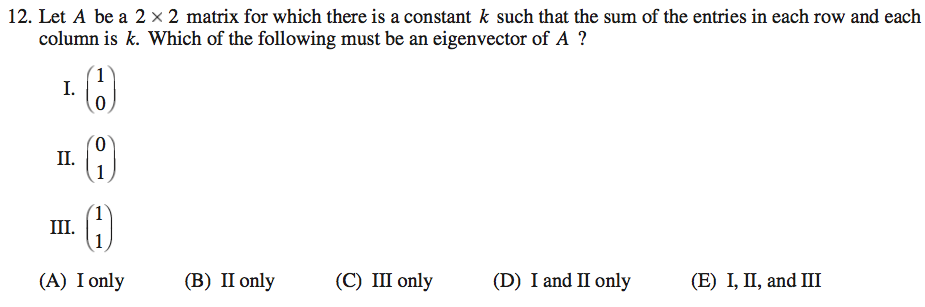
\includegraphics[scale=0.5]{0568_12}

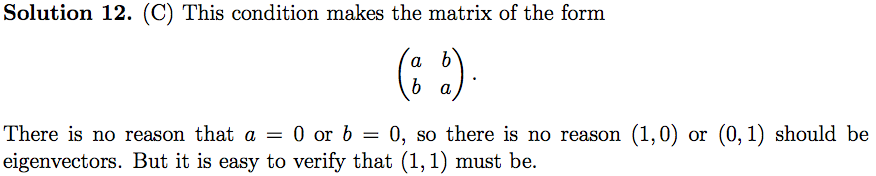
\includegraphics[scale=0.5]{0568_12s}

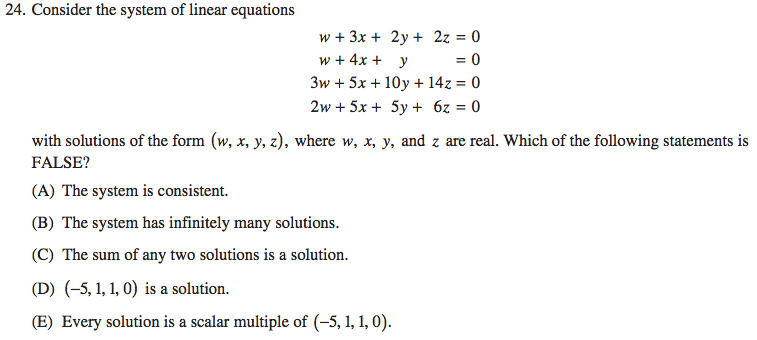
\includegraphics[scale=0.65]{1268_24}

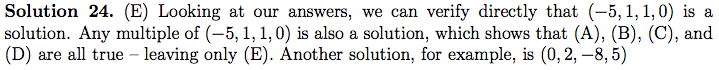
\includegraphics[scale=0.65]{1268_24s}

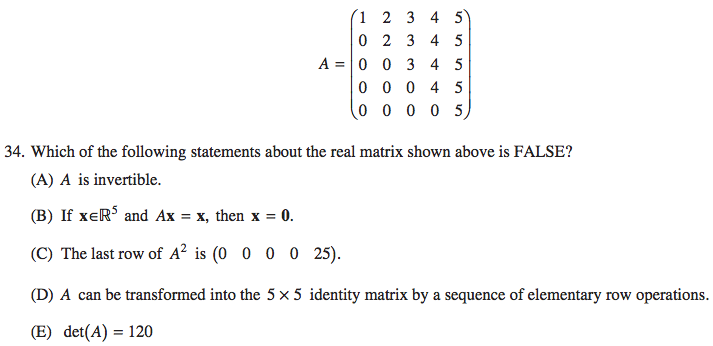
\includegraphics[scale=0.65]{1268_34}

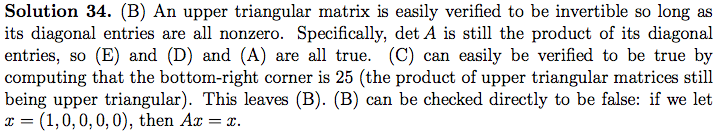
\includegraphics[scale=0.65]{1268_34s}

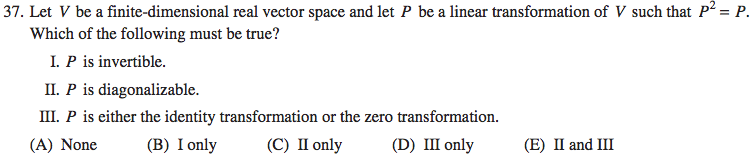
\includegraphics[scale=0.65]{1268_37}

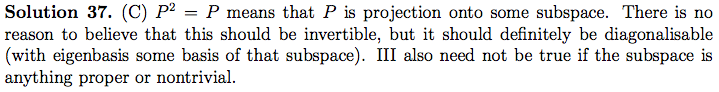
\includegraphics[scale=0.65]{1268_37s}

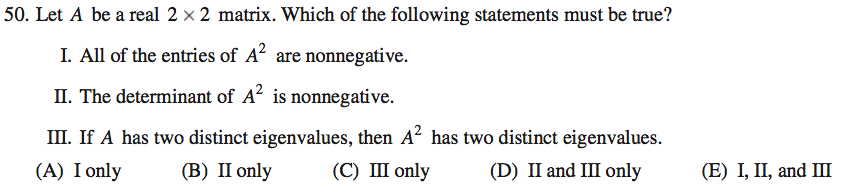
\includegraphics[scale=0.5]{0568_50}

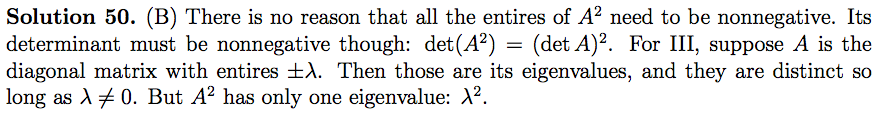
\includegraphics[scale=0.5]{0568_50s}

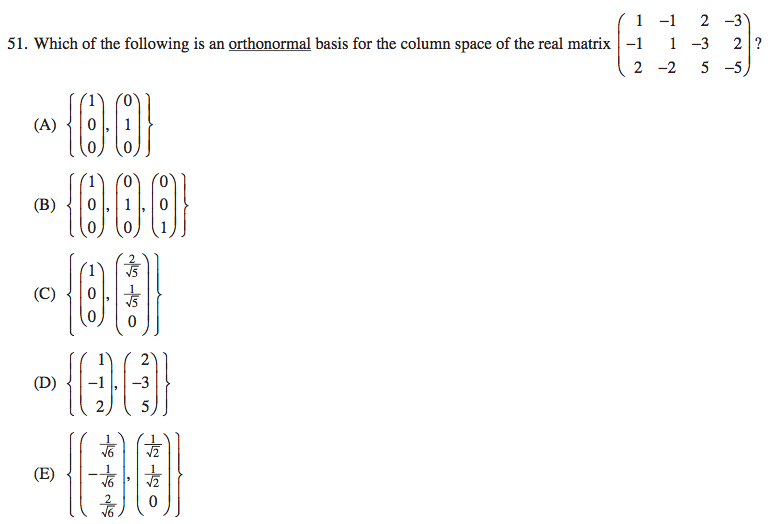
\includegraphics[scale=0.65]{1268_51}

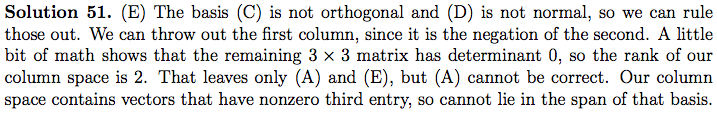
\includegraphics[scale=0.65]{1268_51s}

%%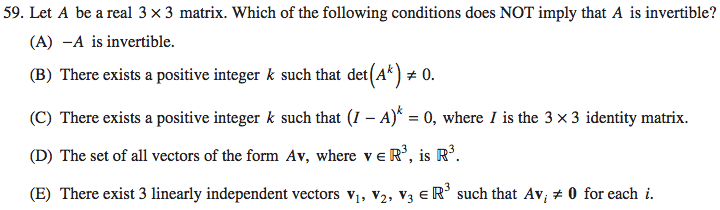
\includegraphics[scale=0.65]{1268_59}
%
%%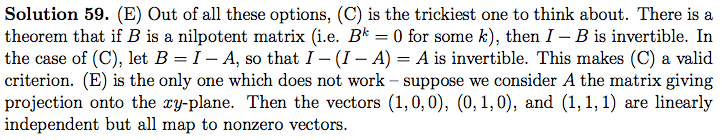
\includegraphics[scale=0.65]{1268_59s}

%
%
%
%
%

%\end{document}



